\PassOptionsToPackage{unicode=true}{hyperref} % options for packages loaded elsewhere
\PassOptionsToPackage{hyphens}{url}
%
\documentclass[]{article}
\usepackage{lmodern}
\usepackage{amssymb,amsmath}
\usepackage{ifxetex,ifluatex}
\usepackage{fixltx2e} % provides \textsubscript
\ifnum 0\ifxetex 1\fi\ifluatex 1\fi=0 % if pdftex
  \usepackage[T1]{fontenc}
  \usepackage[utf8]{inputenc}
  \usepackage{textcomp} % provides euro and other symbols
\else % if luatex or xelatex
  \usepackage{unicode-math}
  \defaultfontfeatures{Ligatures=TeX,Scale=MatchLowercase}
\fi
% use upquote if available, for straight quotes in verbatim environments
\IfFileExists{upquote.sty}{\usepackage{upquote}}{}
% use microtype if available
\IfFileExists{microtype.sty}{%
\usepackage[]{microtype}
\UseMicrotypeSet[protrusion]{basicmath} % disable protrusion for tt fonts
}{}
\IfFileExists{parskip.sty}{%
\usepackage{parskip}
}{% else
\setlength{\parindent}{0pt}
\setlength{\parskip}{6pt plus 2pt minus 1pt}
}
\usepackage{hyperref}
\hypersetup{
            pdftitle={Topic 2: Exercise 1},
            pdfauthor={Daniel Alonso},
            pdfborder={0 0 0},
            breaklinks=true}
\urlstyle{same}  % don't use monospace font for urls
\usepackage[margin=1in]{geometry}
\usepackage{color}
\usepackage{fancyvrb}
\newcommand{\VerbBar}{|}
\newcommand{\VERB}{\Verb[commandchars=\\\{\}]}
\DefineVerbatimEnvironment{Highlighting}{Verbatim}{commandchars=\\\{\}}
% Add ',fontsize=\small' for more characters per line
\usepackage{framed}
\definecolor{shadecolor}{RGB}{248,248,248}
\newenvironment{Shaded}{\begin{snugshade}}{\end{snugshade}}
\newcommand{\AlertTok}[1]{\textcolor[rgb]{0.94,0.16,0.16}{#1}}
\newcommand{\AnnotationTok}[1]{\textcolor[rgb]{0.56,0.35,0.01}{\textbf{\textit{#1}}}}
\newcommand{\AttributeTok}[1]{\textcolor[rgb]{0.77,0.63,0.00}{#1}}
\newcommand{\BaseNTok}[1]{\textcolor[rgb]{0.00,0.00,0.81}{#1}}
\newcommand{\BuiltInTok}[1]{#1}
\newcommand{\CharTok}[1]{\textcolor[rgb]{0.31,0.60,0.02}{#1}}
\newcommand{\CommentTok}[1]{\textcolor[rgb]{0.56,0.35,0.01}{\textit{#1}}}
\newcommand{\CommentVarTok}[1]{\textcolor[rgb]{0.56,0.35,0.01}{\textbf{\textit{#1}}}}
\newcommand{\ConstantTok}[1]{\textcolor[rgb]{0.00,0.00,0.00}{#1}}
\newcommand{\ControlFlowTok}[1]{\textcolor[rgb]{0.13,0.29,0.53}{\textbf{#1}}}
\newcommand{\DataTypeTok}[1]{\textcolor[rgb]{0.13,0.29,0.53}{#1}}
\newcommand{\DecValTok}[1]{\textcolor[rgb]{0.00,0.00,0.81}{#1}}
\newcommand{\DocumentationTok}[1]{\textcolor[rgb]{0.56,0.35,0.01}{\textbf{\textit{#1}}}}
\newcommand{\ErrorTok}[1]{\textcolor[rgb]{0.64,0.00,0.00}{\textbf{#1}}}
\newcommand{\ExtensionTok}[1]{#1}
\newcommand{\FloatTok}[1]{\textcolor[rgb]{0.00,0.00,0.81}{#1}}
\newcommand{\FunctionTok}[1]{\textcolor[rgb]{0.00,0.00,0.00}{#1}}
\newcommand{\ImportTok}[1]{#1}
\newcommand{\InformationTok}[1]{\textcolor[rgb]{0.56,0.35,0.01}{\textbf{\textit{#1}}}}
\newcommand{\KeywordTok}[1]{\textcolor[rgb]{0.13,0.29,0.53}{\textbf{#1}}}
\newcommand{\NormalTok}[1]{#1}
\newcommand{\OperatorTok}[1]{\textcolor[rgb]{0.81,0.36,0.00}{\textbf{#1}}}
\newcommand{\OtherTok}[1]{\textcolor[rgb]{0.56,0.35,0.01}{#1}}
\newcommand{\PreprocessorTok}[1]{\textcolor[rgb]{0.56,0.35,0.01}{\textit{#1}}}
\newcommand{\RegionMarkerTok}[1]{#1}
\newcommand{\SpecialCharTok}[1]{\textcolor[rgb]{0.00,0.00,0.00}{#1}}
\newcommand{\SpecialStringTok}[1]{\textcolor[rgb]{0.31,0.60,0.02}{#1}}
\newcommand{\StringTok}[1]{\textcolor[rgb]{0.31,0.60,0.02}{#1}}
\newcommand{\VariableTok}[1]{\textcolor[rgb]{0.00,0.00,0.00}{#1}}
\newcommand{\VerbatimStringTok}[1]{\textcolor[rgb]{0.31,0.60,0.02}{#1}}
\newcommand{\WarningTok}[1]{\textcolor[rgb]{0.56,0.35,0.01}{\textbf{\textit{#1}}}}
\usepackage{graphicx,grffile}
\makeatletter
\def\maxwidth{\ifdim\Gin@nat@width>\linewidth\linewidth\else\Gin@nat@width\fi}
\def\maxheight{\ifdim\Gin@nat@height>\textheight\textheight\else\Gin@nat@height\fi}
\makeatother
% Scale images if necessary, so that they will not overflow the page
% margins by default, and it is still possible to overwrite the defaults
% using explicit options in \includegraphics[width, height, ...]{}
\setkeys{Gin}{width=\maxwidth,height=\maxheight,keepaspectratio}
\setlength{\emergencystretch}{3em}  % prevent overfull lines
\providecommand{\tightlist}{%
  \setlength{\itemsep}{0pt}\setlength{\parskip}{0pt}}
\setcounter{secnumdepth}{0}
% Redefines (sub)paragraphs to behave more like sections
\ifx\paragraph\undefined\else
\let\oldparagraph\paragraph
\renewcommand{\paragraph}[1]{\oldparagraph{#1}\mbox{}}
\fi
\ifx\subparagraph\undefined\else
\let\oldsubparagraph\subparagraph
\renewcommand{\subparagraph}[1]{\oldsubparagraph{#1}\mbox{}}
\fi

% set default figure placement to htbp
\makeatletter
\def\fps@figure{htbp}
\makeatother


\title{Topic 2: Exercise 1}
\author{Daniel Alonso}
\date{November 28th, 2020}

\begin{document}
\maketitle

\hypertarget{importing-libraries}{%
\paragraph{Importing libraries}\label{importing-libraries}}

\begin{Shaded}
\begin{Highlighting}[]
\KeywordTok{library}\NormalTok{(dplyr)}
\KeywordTok{library}\NormalTok{(Rcpp)}
\KeywordTok{library}\NormalTok{(JuliaCall)}
\end{Highlighting}
\end{Shaded}

\hypertarget{importing-data-as-described-by-exercise}{%
\paragraph{Importing data as described by
exercise}\label{importing-data-as-described-by-exercise}}

\begin{Shaded}
\begin{Highlighting}[]
\NormalTok{d <-}\StringTok{ }\KeywordTok{read.csv}\NormalTok{(}\StringTok{"../../datasets/Colleges.csv"}\NormalTok{)}
\end{Highlighting}
\end{Shaded}

\hypertarget{replacing-binary-variable-private-with-1-and-0}{%
\paragraph{Replacing binary variable Private with 1 and
0}\label{replacing-binary-variable-private-with-1-and-0}}

\begin{Shaded}
\begin{Highlighting}[]
\NormalTok{d}\OperatorTok{$}\NormalTok{Private <-}\StringTok{ }\KeywordTok{ifelse}\NormalTok{(d}\OperatorTok{$}\NormalTok{Private }\OperatorTok{==}\StringTok{ "Yes"}\NormalTok{, }\DecValTok{1}\NormalTok{, }\DecValTok{0}\NormalTok{)}
\end{Highlighting}
\end{Shaded}

\hypertarget{selecting-columns}{%
\paragraph{Selecting columns}\label{selecting-columns}}

\begin{Shaded}
\begin{Highlighting}[]
\NormalTok{data <-}\StringTok{ }\NormalTok{d }\OperatorTok\StringTok{ }\NormalTok{dplyr}\OperatorTok{::}\KeywordTok{select}\NormalTok{(}\StringTok{'Private'}\NormalTok{,}\StringTok{'Apps'}\NormalTok{,}\StringTok{'Accept'}\NormalTok{,}\StringTok{'Enroll'}\NormalTok{,}\StringTok{'F.Undergrad'}\NormalTok{)}
\end{Highlighting}
\end{Shaded}

\hypertarget{calculating-covariances}{%
\paragraph{Calculating covariances}\label{calculating-covariances}}

\begin{Shaded}
\begin{Highlighting}[]
\NormalTok{cov_matrix <-}\StringTok{ }\KeywordTok{cov}\NormalTok{(data)}
\NormalTok{cov_matrix}
\CommentTok{#>                   Private          Apps        Accept       Enroll  F.Undergrad}
\CommentTok{#> Private         0.1986559     -745.3552     -519.2042    -235.1942    -1330.764}
\CommentTok{#> Apps         -745.3552439 14978459.5301  8949859.8119 3045255.9876 15289702.474}
\CommentTok{#> Accept       -519.2042169  8949859.8119  6007959.6988 2076267.7627 10393582.435}
\CommentTok{#> Enroll       -235.1942393  3045255.9876  2076267.7627  863368.3923  4347529.884}
\CommentTok{#> F.Undergrad -1330.7637175 15289702.4742 10393582.4355 4347529.8841 23526579.326}
\end{Highlighting}
\end{Shaded}

\newpage

\hypertarget{calculating-correlations}{%
\paragraph{Calculating correlations}\label{calculating-correlations}}

\begin{Shaded}
\begin{Highlighting}[]
\NormalTok{corr_matrix <-}\StringTok{ }\KeywordTok{cov2cor}\NormalTok{(cov_matrix)}
\NormalTok{corr_matrix}
\CommentTok{#>                Private       Apps     Accept     Enroll F.Undergrad}
\CommentTok{#> Private      1.0000000 -0.4320947 -0.4752520 -0.5679078  -0.6155605}
\CommentTok{#> Apps        -0.4320947  1.0000000  0.9434506  0.8468221   0.8144906}
\CommentTok{#> Accept      -0.4752520  0.9434506  1.0000000  0.9116367   0.8742233}
\CommentTok{#> Enroll      -0.5679078  0.8468221  0.9116367  1.0000000   0.9646397}
\CommentTok{#> F.Undergrad -0.6155605  0.8144906  0.8742233  0.9646397   1.0000000}
\end{Highlighting}
\end{Shaded}

\hypertarget{experimenting-a-little-bit-with-the-private-variable}{%
\paragraph{Experimenting a little bit with the private
variable}\label{experimenting-a-little-bit-with-the-private-variable}}

Let's try changing the Yes to 0 and the No to 1 and checking the
covariances and correlations

\begin{Shaded}
\begin{Highlighting}[]
\NormalTok{d <-}\StringTok{ }\KeywordTok{read.csv}\NormalTok{(}\StringTok{"../../datasets/Colleges.csv"}\NormalTok{)}
\NormalTok{d}\OperatorTok{$}\NormalTok{Private <-}\StringTok{ }\KeywordTok{ifelse}\NormalTok{(d}\OperatorTok{$}\NormalTok{Private }\OperatorTok{==}\StringTok{ "Yes"}\NormalTok{, }\DecValTok{0}\NormalTok{, }\DecValTok{1}\NormalTok{)}
\NormalTok{data <-}\StringTok{ }\NormalTok{d }\OperatorTok\StringTok{ }\NormalTok{dplyr}\OperatorTok{::}\KeywordTok{select}\NormalTok{(}\StringTok{'Private'}\NormalTok{,}\StringTok{'Apps'}\NormalTok{,}\StringTok{'Accept'}\NormalTok{,}\StringTok{'Enroll'}\NormalTok{,}\StringTok{'F.Undergrad'}\NormalTok{)}
\end{Highlighting}
\end{Shaded}

\begin{Shaded}
\begin{Highlighting}[]
\NormalTok{cov_matrix <-}\StringTok{ }\KeywordTok{cov}\NormalTok{(data)}
\NormalTok{cov_matrix}
\CommentTok{#>                  Private         Apps       Accept       Enroll  F.Undergrad}
\CommentTok{#> Private        0.1986559 7.453552e+02 5.192042e+02     235.1942     1330.764}
\CommentTok{#> Apps         745.3552439 1.497846e+07 8.949860e+06 3045255.9876 15289702.474}
\CommentTok{#> Accept       519.2042169 8.949860e+06 6.007960e+06 2076267.7627 10393582.435}
\CommentTok{#> Enroll       235.1942393 3.045256e+06 2.076268e+06  863368.3923  4347529.884}
\CommentTok{#> F.Undergrad 1330.7637175 1.528970e+07 1.039358e+07 4347529.8841 23526579.326}
\NormalTok{corr_matrix <-}\StringTok{ }\KeywordTok{cov2cor}\NormalTok{(cov_matrix)}
\NormalTok{corr_matrix}
\CommentTok{#>               Private      Apps    Accept    Enroll F.Undergrad}
\CommentTok{#> Private     1.0000000 0.4320947 0.4752520 0.5679078   0.6155605}
\CommentTok{#> Apps        0.4320947 1.0000000 0.9434506 0.8468221   0.8144906}
\CommentTok{#> Accept      0.4752520 0.9434506 1.0000000 0.9116367   0.8742233}
\CommentTok{#> Enroll      0.5679078 0.8468221 0.9116367 1.0000000   0.9646397}
\CommentTok{#> F.Undergrad 0.6155605 0.8144906 0.8742233 0.9646397   1.0000000}
\end{Highlighting}
\end{Shaded}

We get the same numbers with reversed signs.

\newpage

\hypertarget{we-define-the-following-function-in-julia-to-help-our-understanding}{%
\subsubsection{We define the following function (in julia) to help our
understanding:}\label{we-define-the-following-function-in-julia-to-help-our-understanding}}

Takes the arguments:

\begin{verbatim}
- nrows: number of data to simulate (amount of rows)
- simulations: number of different times to simulate and average the results
- fixed_value_col: boolean parameter with true -> assigns a set of values between mins[1] and maxs[1] (other 2 parameters)
- reverse: boolean parameter that determines whether the 0s in the binary variable are assigned to the higher values or not
- sim_binaries: this would simulate a rolling proportion of binaries where iteration 1 has all zeros in the binary variable and iteration *nrows* has all 1s in the binary variable
- mins: array containing as first element the minimum value to use for corresponding values in the quantitative columns with 1s and 0s assuming the fixed_value_col parameter is set to false, if it's set to true then it'll be the minimum of the quantitative variable we are calculating the covariance or correlation vs the quantitative variable. the second element of the array represents the same minimum but for the 2nd array which will substitute the values of elements that are 1 or 0 depending on the user choice. (for example: if reverse=false, fixed_value_col=false, maxs=[10,10000] and mins=[1,100],  the values in the quantitative variable corresponding to 1s in the binary variable will, as the loop goes on, go from having minimum value 1 to minimum value 100 and with will go from having maximum value 10 to maximum value 10000, therefore assigning high values (between 100-10000) to elements in the quant.variable corresponding to 1 in the binary variable and keep lower values (between 1-10) for the ones corresponding to 0s in the binary variable)
- maxs: same as minimum but they're the maximums.
\end{verbatim}

Example of how the dataset changes for a run of the function with
parameters: nrows=5, simulations=1 and the rest of the parameters as
default:

\begin{figure}
\centering
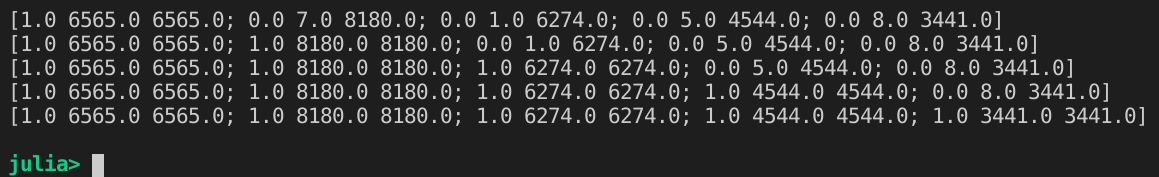
\includegraphics{julia_output.png}
\caption{Example of a simulated dataset with the function
simulation\_general in the Julia REPL}
\end{figure}

In Figure 1 we can see 5 iterations (as there's 5 simulated rows) using
the function, where the leftmost value of each row is a binary variable
(1 or 0), starting with (1,0,0,0,0) and ending with (1,1,1,1,1), and for
our quantitative variable (with which we will calculate cov/corr) we can
see the values go from a high value (copied from the 3rd column) and the
rest of values being small (6565,7,1,5,8) and ending with large values
(copied from column 3) being (6565, 8180, 6214, 4544, 3441).

\hypertarget{function-definition}{%
\subsubsection{Function definition}\label{function-definition}}

\begin{Shaded}
\begin{Highlighting}[]
\NormalTok{using Random}
\NormalTok{using Statistics}
\NormalTok{using Plots}
\NormalTok{gr()}
\CommentTok{#> Plots.GRBackend()}

\KeywordTok{function}\NormalTok{ simulation_general(nrows, simulations; fixed_value_col=false, }
\NormalTok{    reverse=false, sim_binaries=true, mins=[}\FloatTok{1}\NormalTok{,}\FloatTok{100}\NormalTok{], maxs=[}\FloatTok{10}\NormalTok{,}\FloatTok{10000}\NormalTok{]) }
    \CommentTok{# cov and corr matrixes}
\NormalTok{    covs = zeros(}\DataTypeTok{Float64}\NormalTok{, nrows, simulations)}
\NormalTok{    corr = zeros(}\DataTypeTok{Float64}\NormalTok{, nrows, simulations)}

    \CommentTok{# loop}
    \KeywordTok{for}\NormalTok{ s }\KeywordTok{in} \FloatTok{1}\NormalTok{:simulations}
\NormalTok{        pvtapps = zeros(}\DataTypeTok{Float64}\NormalTok{, nrows, }\FloatTok{3}\NormalTok{)}
        \KeywordTok{if}\NormalTok{ sim_binaries == false}
\NormalTok{            pvtapps[:,}\FloatTok{1}\NormalTok{] = rand(}\FloatTok{0}\NormalTok{:}\FloatTok{1}\NormalTok{, nrows)}
        \KeywordTok{end}

        \CommentTok{# random numbers column (quant variable)}
        \KeywordTok{if}\NormalTok{ fixed_value_col == true}
\NormalTok{            pvtapps[:,}\FloatTok{2}\NormalTok{] = rand(mins[}\FloatTok{1}\NormalTok{]:maxs[}\FloatTok{1}\NormalTok{],nrows)}
        \KeywordTok{else}
            \KeywordTok{if}\NormalTok{ reverse == false}
\NormalTok{                pvtapps[:,}\FloatTok{2}\NormalTok{] = rand(mins[}\FloatTok{1}\NormalTok{]:maxs[}\FloatTok{1}\NormalTok{],nrows)}
\NormalTok{                pvtapps[:,}\FloatTok{3}\NormalTok{] = rand(mins[}\FloatTok{2}\NormalTok{]:maxs[}\FloatTok{2}\NormalTok{],nrows)}
            \KeywordTok{else} 
\NormalTok{                pvtapps[:,}\FloatTok{3}\NormalTok{] = rand(mins[}\FloatTok{1}\NormalTok{]:maxs[}\FloatTok{1}\NormalTok{],nrows)}
\NormalTok{                pvtapps[:,}\FloatTok{2}\NormalTok{] = rand(mins[}\FloatTok{2}\NormalTok{]:maxs[}\FloatTok{2}\NormalTok{],nrows)}
            \KeywordTok{end}
        \KeywordTok{end}

        \CommentTok{# loop for changing values}
        \KeywordTok{for}\NormalTok{ i }\KeywordTok{in} \FloatTok{1}\NormalTok{:nrows}

            \CommentTok{# rolling binary proportions}
            \KeywordTok{if}\NormalTok{ sim_binaries == true}
\NormalTok{                pvtapps[}\FloatTok{1}\NormalTok{:i,}\FloatTok{1}\NormalTok{] = ones(i)}
            \KeywordTok{end}

            \CommentTok{# replacing values by larger/smaller ones in col2}
            \KeywordTok{if}\NormalTok{ fixed_value_col == false}
\NormalTok{                pvtapps[}\FloatTok{1}\NormalTok{:i,}\FloatTok{2}\NormalTok{] = pvtapps[}\FloatTok{1}\NormalTok{:i,}\FloatTok{3}\NormalTok{]}
            \KeywordTok{end}
            \CommentTok{# calculate corr and cov}
\NormalTok{            covs[i,s] = cov(pvtapps[:,}\FloatTok{1}\NormalTok{],pvtapps[:,}\FloatTok{2}\NormalTok{])}
\NormalTok{            corr[i,s] = cor(pvtapps[:,}\FloatTok{1}\NormalTok{],pvtapps[:,}\FloatTok{2}\NormalTok{])}
        \KeywordTok{end}
    \KeywordTok{end}

    \CommentTok{# results}
\NormalTok{    covsrows = zeros(}\DataTypeTok{Float64}\NormalTok{, nrows)}
\NormalTok{    corrrows = zeros(}\DataTypeTok{Float64}\NormalTok{, nrows)}
    \KeywordTok{for}\NormalTok{ i }\KeywordTok{in} \FloatTok{1}\NormalTok{:nrows}
\NormalTok{        covsrows[i] = mean(covs[i,:])}
\NormalTok{        corrrows[i] = mean(corr[i,:])}
    \KeywordTok{end}

    \CommentTok{# return matrixes}
    \KeywordTok{return}\NormalTok{ covsrows, corrrows}
\KeywordTok{end}
\CommentTok{#> simulation_general (generic function with 1 method)}
\end{Highlighting}
\end{Shaded}

\begin{Shaded}
\begin{Highlighting}[]
\NormalTok{covsrows, corrrows = simulation_general(}\FloatTok{500}\NormalTok{,}\FloatTok{200}\NormalTok{, reverse=false, sim_binaries=true);}
\end{Highlighting}
\end{Shaded}

\newpage

\hypertarget{covariance-plots-with-500-data-points-and-200-simulations-averaged}{%
\subsubsection{Covariance plots with 500 data points and 200 simulations
averaged}\label{covariance-plots-with-500-data-points-and-200-simulations-averaged}}

\hypertarget{first-scenario-larger-numbers-correspond-to-1s}{%
\paragraph{First scenario: larger numbers correspond to
1s}\label{first-scenario-larger-numbers-correspond-to-1s}}

\begin{Shaded}
\begin{Highlighting}[]
\NormalTok{covsrows <-}\StringTok{ }\NormalTok{JuliaCall}\OperatorTok{::}\KeywordTok{julia_eval}\NormalTok{(}\StringTok{"covsrows"}\NormalTok{)}
\KeywordTok{plot}\NormalTok{(covsrows)}
\end{Highlighting}
\end{Shaded}

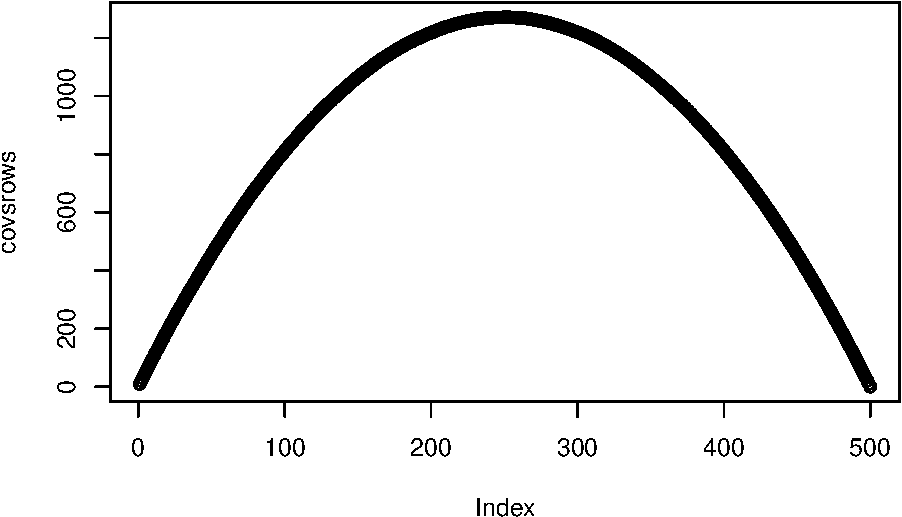
\includegraphics{./figures/unnamed-chunk-11-1.pdf}

Each point here corresponds to one iteration of the function (leftmost
being an iteration where the binary variable had its first value as 1
and the rest as 0 and rightmost being all 1s). For each 1 in the binary
variable we have a value between 100 and 10000 in the quantitative
variable used to calculate the covariance. For each 0 we have a value
between 1 and 10, therefore, all values in the quantitative variable
corresponding to a 0 in the binary are at least an order (x10) of
magnitude larger than those corresponding to a 1.

Clearly, as long as values in the quantitative variable (corresponding
to 1 in the binary variable) remain significantly larger than those
corresponding to 0 the 0 in the binary variable, our covariance will
grow as the proportion of 1s grow, however, once we reach half and half
(half 0s and half 1s in the binary variable), our function reaches its
global maximum and becomes a decreasing function.

\newpage

\hypertarget{second-scenario-larger-numbers-correspond-to-0s}{%
\paragraph{Second scenario: larger numbers correspond to
0s}\label{second-scenario-larger-numbers-correspond-to-0s}}

The opposite thing would happen if we reverse the values, so then we
would have the values corresponding to the binary variable's 1 to the
smaller values (1-10) and larger values (100-10000) corresponding to the
binary variable's 0.

\begin{Shaded}
\begin{Highlighting}[]
\NormalTok{covsrows_rev, corrrows_rev = simulation_general(}\FloatTok{500}\NormalTok{,}\FloatTok{200}\NormalTok{, reverse=true, sim_binaries=true);}
\end{Highlighting}
\end{Shaded}

\begin{Shaded}
\begin{Highlighting}[]
\NormalTok{covsrows_rev <-}\StringTok{ }\NormalTok{JuliaCall}\OperatorTok{::}\KeywordTok{julia_eval}\NormalTok{(}\StringTok{"covsrows_rev"}\NormalTok{)}
\KeywordTok{plot}\NormalTok{(covsrows_rev)}
\end{Highlighting}
\end{Shaded}

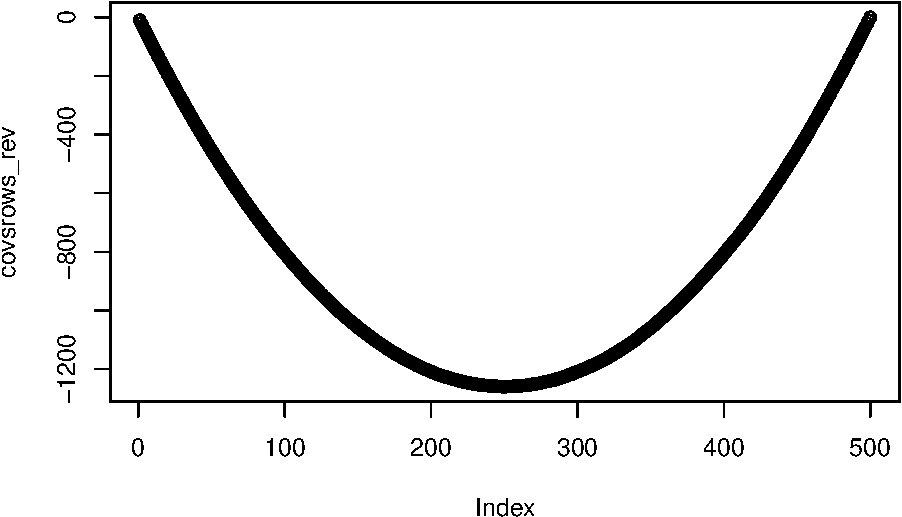
\includegraphics{./figures/unnamed-chunk-13-1.pdf}

\newpage

\hypertarget{third-scenario-just-random-data-and-equal-proportion-of-0s-and-1s}{%
\paragraph{Third scenario: just random data and equal proportion of 0s
and
1s}\label{third-scenario-just-random-data-and-equal-proportion-of-0s-and-1s}}

Here we simulated 700 rows in 500 simulations to have a larger sample to
average the rows with.

If we only simulate without considering the binary variable, so
basically keeping a somewhat even amount of ones and zeros in it and
randomizing the values of the quantitative variable, then we get no
discernible pattern other than (at times) drops around the middle (when
proportions of 0s and 1s are the same) or in the extremes (when the
binary variable is only 1 or 0):

\begin{Shaded}
\begin{Highlighting}[]
\NormalTok{rand_covrows, rand_corrrows = simulation_general(}\FloatTok{700}\NormalTok{,}\FloatTok{500}\NormalTok{, }
\NormalTok{                                        sim_binaries=false, fixed_value_col=false);}
\end{Highlighting}
\end{Shaded}

\begin{Shaded}
\begin{Highlighting}[]
\NormalTok{rand_covrows <-}\StringTok{ }\NormalTok{JuliaCall}\OperatorTok{::}\KeywordTok{julia_eval}\NormalTok{(}\StringTok{"rand_covrows"}\NormalTok{)}
\KeywordTok{plot}\NormalTok{(rand_covrows)}
\end{Highlighting}
\end{Shaded}

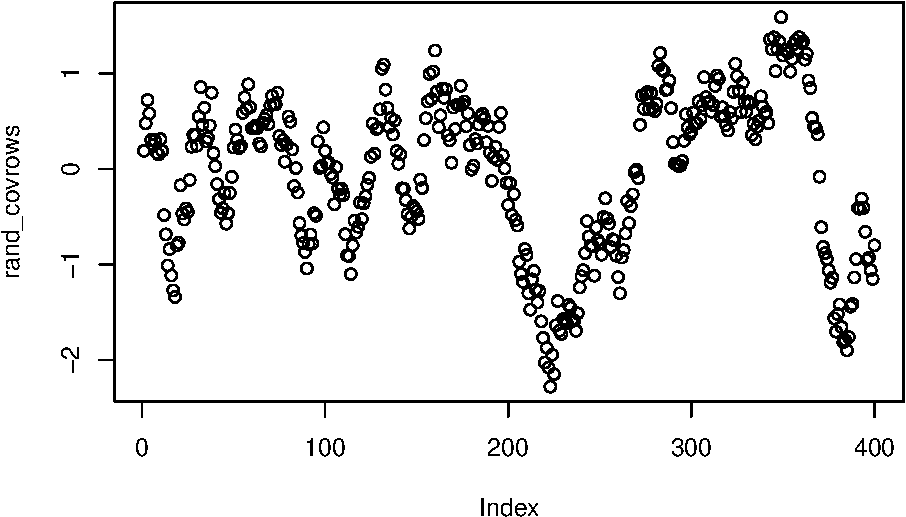
\includegraphics{./figures/unnamed-chunk-15-1.pdf}

\newpage

\hypertarget{correlation-plot-with-500-data-points-and-200-simulations-averaged}{%
\subsubsection{Correlation plot with 500 data points and 200 simulations
averaged}\label{correlation-plot-with-500-data-points-and-200-simulations-averaged}}

\hypertarget{first-scenario-larger-numbers-correspond-to-1s-1}{%
\paragraph{First scenario: larger numbers correspond to
1s}\label{first-scenario-larger-numbers-correspond-to-1s-1}}

\begin{Shaded}
\begin{Highlighting}[]
\NormalTok{corrrows <-}\StringTok{ }\NormalTok{JuliaCall}\OperatorTok{::}\KeywordTok{julia_eval}\NormalTok{(}\StringTok{"corrrows"}\NormalTok{)}
\KeywordTok{plot}\NormalTok{(corrrows)}
\end{Highlighting}
\end{Shaded}

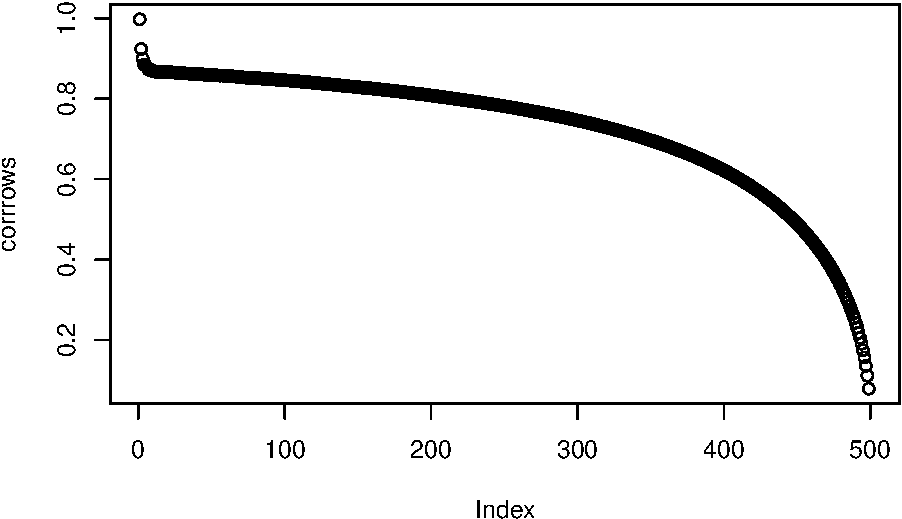
\includegraphics{./figures/unnamed-chunk-16-1.pdf}

here we can see that while values for the 1s are higher than values for
the 0s and while the proportion of 0s remains larger than the proportion
of 1s, the correlation stays relatively high. When the proportion of 1s
becomes higher than the proportion of 0s, then the correlation starts to
drop and quickly approaches zero.

The correlation has its maximum value when the binary variable is
basically all zeros (only a single 1 in it) and reaches its minimum
value when all the values in in the binary variable are 1s.

\newpage

\hypertarget{second-scenario-larger-numbers-correspond-to-0s-1}{%
\paragraph{Second scenario: larger numbers correspond to
0s}\label{second-scenario-larger-numbers-correspond-to-0s-1}}

Something quite similar but contrary to the previous situation happens
with correlation when the opposite scenario occurs. Basically, our
minimum value will be the highest correlation (as all the correlations
here are negative). The highest correlation (minimum value in the plot
for the y axis) happens when all our data points in the binary variable
are 1s and all the values for the quantitative variable have been
replaced by higher numbers (as here, the higher values in the
quantitative variables correspond to the zeros in the binary variable).

The minimum correlation (\textasciitilde{}0) is reached right at the
start, when all the values for the binary variable are 0s (except for a
single value).

\begin{Shaded}
\begin{Highlighting}[]
\NormalTok{corrrows_rev <-}\StringTok{ }\NormalTok{JuliaCall}\OperatorTok{::}\KeywordTok{julia_eval}\NormalTok{(}\StringTok{"corrrows_rev"}\NormalTok{)}
\KeywordTok{plot}\NormalTok{(corrrows_rev)}
\end{Highlighting}
\end{Shaded}

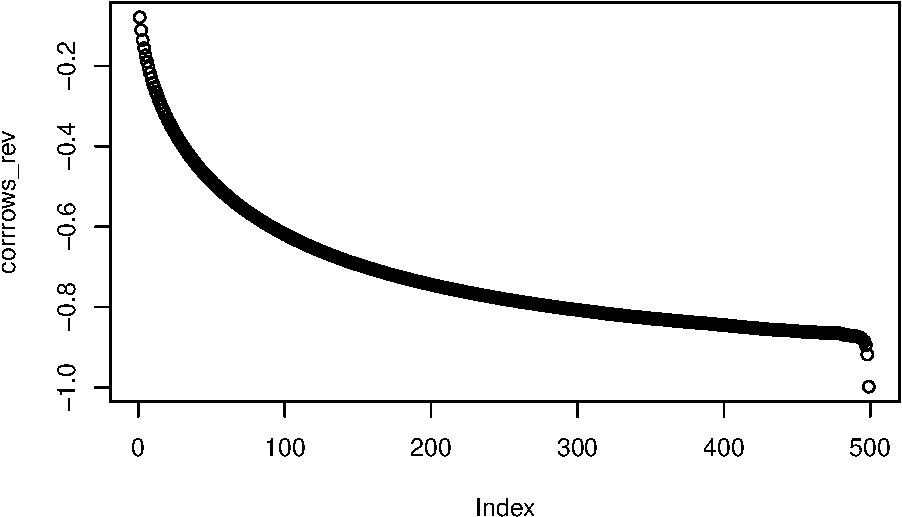
\includegraphics{./figures/unnamed-chunk-17-1.pdf}

\newpage

\hypertarget{third-scenario-just-random-data-and-equal-proportion-of-0s-and-1s-1}{%
\paragraph{Third scenario: just random data and equal proportion of 0s
and
1s}\label{third-scenario-just-random-data-and-equal-proportion-of-0s-and-1s-1}}

For randomized data with different values in every simulation we get
essentially the same thing we saw with covariance. No discernible
pattern and the plot will change every time it's made, as it's
\emph{just random data} averaged.

\begin{Shaded}
\begin{Highlighting}[]
\NormalTok{rand_corrrows <-}\StringTok{ }\NormalTok{JuliaCall}\OperatorTok{::}\KeywordTok{julia_eval}\NormalTok{(}\StringTok{"rand_corrrows"}\NormalTok{)}
\KeywordTok{plot}\NormalTok{(rand_corrrows)}
\end{Highlighting}
\end{Shaded}

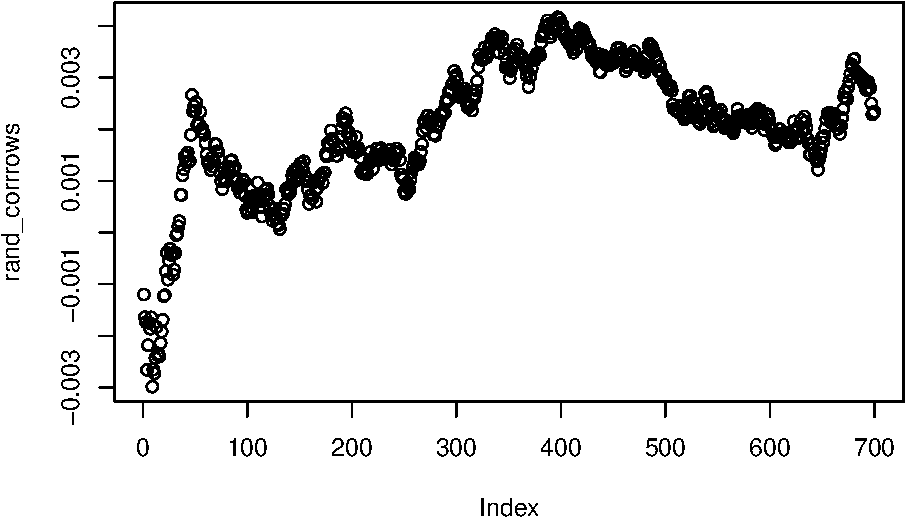
\includegraphics{./figures/unnamed-chunk-18-1.pdf}

\newpage

\hypertarget{fourth-scenario-quantitative-variable-with-only-negative-values}{%
\paragraph{Fourth scenario: quantitative variable with only negative
values}\label{fourth-scenario-quantitative-variable-with-only-negative-values}}

Very similarly to the scenario with only positive values but the
opposite. So basically our correlations are negative and we start with a
lower correlation to increase rapidly and then we drop back again
rapidly after the proportion of 1s and 0s is around 75\% 1s and 25\% 0s.

\begin{Shaded}
\begin{Highlighting}[]
\NormalTok{_, corrrows_neg = simulation_general(}\FloatTok{500}\NormalTok{,}\FloatTok{200}\NormalTok{, mins=[-}\FloatTok{100}\NormalTok{,-}\FloatTok{1000}\NormalTok{], maxs=[-}\FloatTok{10}\NormalTok{,-}\FloatTok{200}\NormalTok{]);}
\end{Highlighting}
\end{Shaded}

\begin{Shaded}
\begin{Highlighting}[]
\NormalTok{corrrows_neg <-}\StringTok{ }\NormalTok{JuliaCall}\OperatorTok{::}\KeywordTok{julia_eval}\NormalTok{(}\StringTok{"corrrows_neg"}\NormalTok{)}
\KeywordTok{plot}\NormalTok{(corrrows_neg)}
\end{Highlighting}
\end{Shaded}

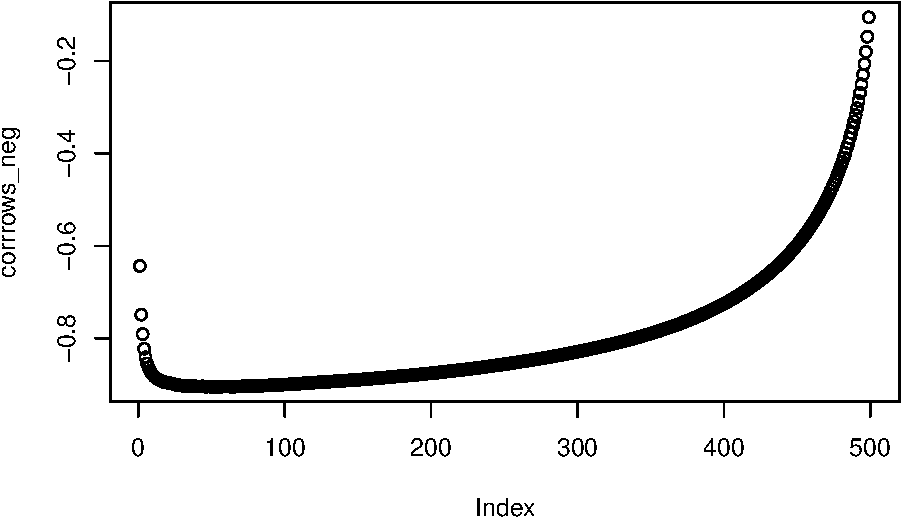
\includegraphics{./figures/unnamed-chunk-20-1.pdf}

\newpage

\hypertarget{fifth-scenario-quantitative-variable-with-only-negative-values-in-reverse}{%
\paragraph{Fifth scenario: quantitative variable with only negative
values (in
reverse)}\label{fifth-scenario-quantitative-variable-with-only-negative-values-in-reverse}}

Essentially the same as the fourth scenario but flipped.

\begin{Shaded}
\begin{Highlighting}[]
\NormalTok{_, corrrows_neg = simulation_general(}\FloatTok{500}\NormalTok{,}\FloatTok{200}\NormalTok{, reverse=true, mins=[-}\FloatTok{100}\NormalTok{,-}\FloatTok{1000}\NormalTok{], maxs=[-}\FloatTok{10}\NormalTok{,-}\FloatTok{200}\NormalTok{]);}
\end{Highlighting}
\end{Shaded}

\begin{Shaded}
\begin{Highlighting}[]
\NormalTok{corrrows_neg <-}\StringTok{ }\NormalTok{JuliaCall}\OperatorTok{::}\KeywordTok{julia_eval}\NormalTok{(}\StringTok{"corrrows_neg"}\NormalTok{)}
\KeywordTok{plot}\NormalTok{(corrrows_neg)}
\end{Highlighting}
\end{Shaded}

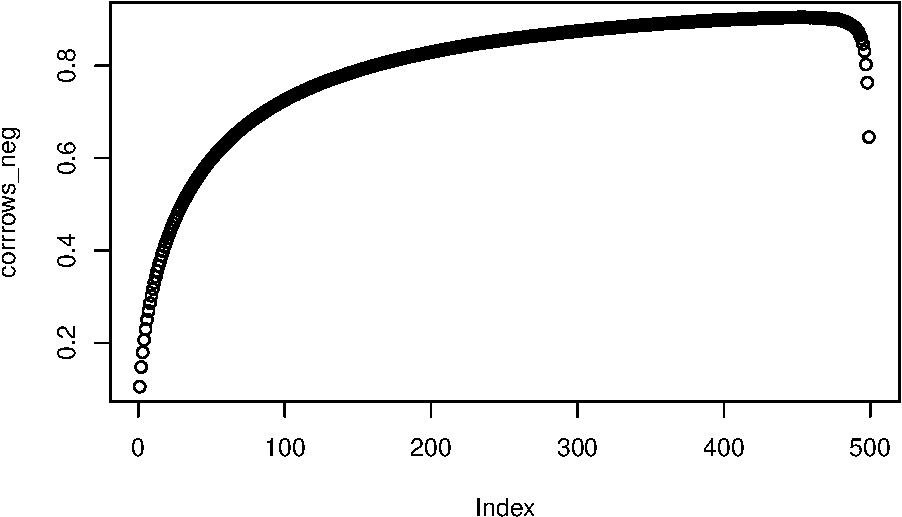
\includegraphics{./figures/unnamed-chunk-22-1.pdf}

\newpage

\hypertarget{sixth-scenario-quantitative-variable-with-both-negative-and-positive-values}{%
\paragraph{Sixth scenario: quantitative variable with both negative and
positive
values}\label{sixth-scenario-quantitative-variable-with-both-negative-and-positive-values}}

Very similar to the fourth scenario but correlation drops much faster
after the proportion of ones and zeros is about the same and our maximum
correlation (\textasciitilde{} -0.7) doesn't reach -1 in this case (as
it does with the previous one).

\begin{Shaded}
\begin{Highlighting}[]
\NormalTok{_, corrrows_both = simulation_general(}\FloatTok{500}\NormalTok{,}\FloatTok{200}\NormalTok{, mins=[-}\FloatTok{100}\NormalTok{,-}\FloatTok{1000}\NormalTok{], maxs=[}\FloatTok{10}\NormalTok{,}\FloatTok{200}\NormalTok{]);}
\end{Highlighting}
\end{Shaded}

\begin{Shaded}
\begin{Highlighting}[]
\NormalTok{corrrows_both <-}\StringTok{ }\NormalTok{JuliaCall}\OperatorTok{::}\KeywordTok{julia_eval}\NormalTok{(}\StringTok{"corrrows_both"}\NormalTok{)}
\KeywordTok{plot}\NormalTok{(corrrows_both)}
\end{Highlighting}
\end{Shaded}

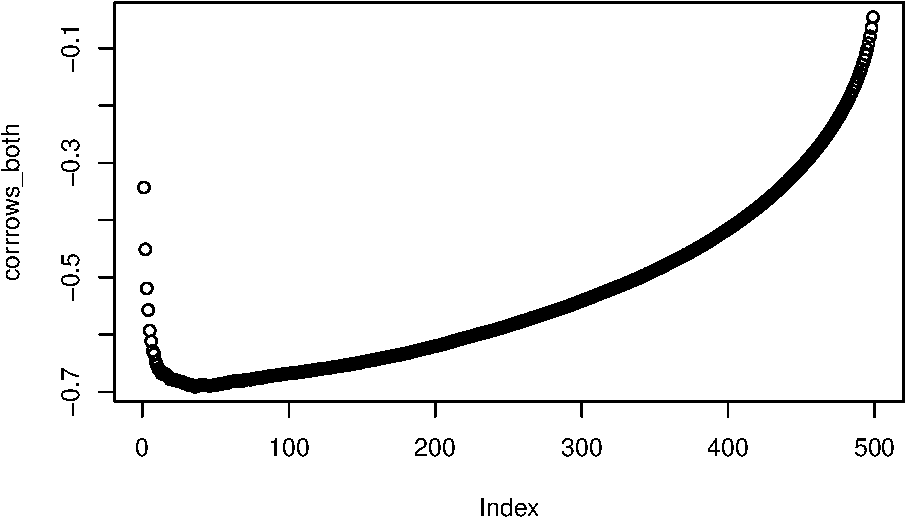
\includegraphics{./figures/unnamed-chunk-24-1.pdf}

\newpage

\hypertarget{seventh-scenario-quantitative-variable-with-both-negative-and-positive-values-in-reverse}{%
\paragraph{Seventh scenario: quantitative variable with both negative
and positive values (in
reverse)}\label{seventh-scenario-quantitative-variable-with-both-negative-and-positive-values-in-reverse}}

Very similar to the sixth scenario but opposite. In both sixth and
seventh scenario, our correlations drop very rapidly when our binary
variable is either (nearly) entirely 1s or 0s.

\begin{Shaded}
\begin{Highlighting}[]
\NormalTok{_, corrrows_both = simulation_general(}\FloatTok{500}\NormalTok{,}\FloatTok{200}\NormalTok{, reverse=true, mins=[-}\FloatTok{100}\NormalTok{,-}\FloatTok{1000}\NormalTok{], maxs=[}\FloatTok{10}\NormalTok{,}\FloatTok{200}\NormalTok{]);}
\end{Highlighting}
\end{Shaded}

\begin{Shaded}
\begin{Highlighting}[]
\NormalTok{corrrows_both <-}\StringTok{ }\NormalTok{JuliaCall}\OperatorTok{::}\KeywordTok{julia_eval}\NormalTok{(}\StringTok{"corrrows_both"}\NormalTok{)}
\KeywordTok{plot}\NormalTok{(corrrows_both)}
\end{Highlighting}
\end{Shaded}

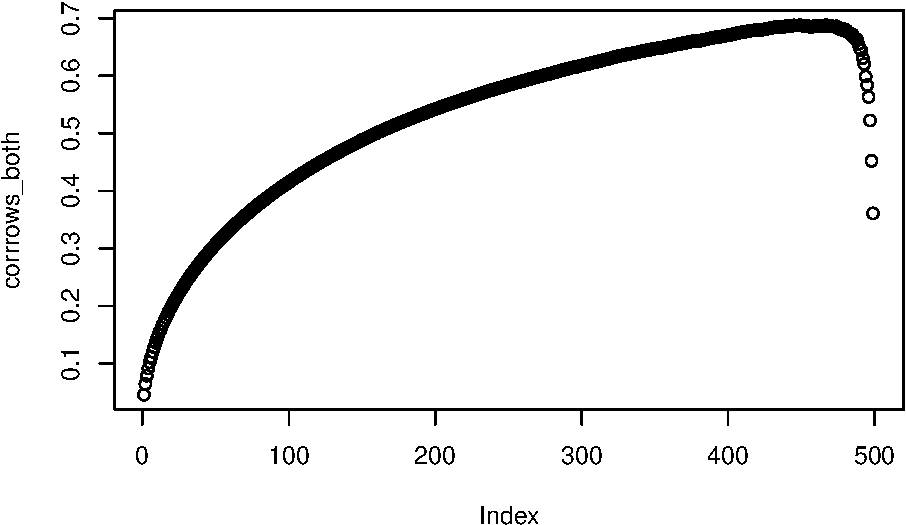
\includegraphics{./figures/unnamed-chunk-26-1.pdf}

\newpage

\hypertarget{what-information-does-the-sample-covariance-provide}{%
\subsection{What information does the sample covariance
provide?}\label{what-information-does-the-sample-covariance-provide}}

From my observations I don't think I can confidently answer this
question and say that this might have an interesting deeper
\emph{meaning}. I don't really see it as clearly as it would be seen
with just 2 ordinary quantitative variables. However, there is
definitely a pattern, when higher values correspond to 1s and the
proportion of 1s and 0s is relatively even, then we have the maximum
covariance we can have, and the opposite will happen in the opposite
scenario.

If we have a covariance close to 0 we can say that that it could be
(according to my testing) due to:

\begin{verbatim}
- There's a significantly higher amount of 0s or 1s in the binary variable
\end{verbatim}

If we have a covariance that is maximized or minimized (vs other
scenarios with a different proportion of 1s and 0s in the binary
variable) then it could be due to a few things:

\begin{verbatim}
- If it's maximized (vs other scenarios):
    - It could be that the higher values correspond to 1s in the binary variable
- If it's minimized (vs other scenarios):
    - It could be that the lower values correspond to 1s in the binary variable
\end{verbatim}

\hypertarget{what-information-does-the-sample-correlation-provide}{%
\subsection{What information does the sample correlation
provide?}\label{what-information-does-the-sample-correlation-provide}}

Similar to covariance, I'm not quite sure if I'm confident enough in my
findings to say that I can give a profound meaning to this correlation.
But I can point out a few observations:

(using only positive values) If correlation is very high (vs other
scenarios) it could be (according to my observations) due to:

\begin{verbatim}
- Higher values in the quantitative variable correspond to 1s in the binary variable and there's 
more 0s than 1s in the binary variable (0s represent more than 40% of the observations)
    - In this case, correlation will be positive
- Higher values in the quantitative variables correspond to 0s in the binary variable and there's
more 1s than 0s in the binary variable (1s represent more than 40% of the observations)
    - In this case, correlation will be negative
\end{verbatim}

(using only negative values) If correlation is very high (vs other
scenarios) it could be (according to my observations) due to:

\begin{verbatim}
- Same conclusions as with positive values only, however, correlation drops when the total 
amount of 1s and 0s replace the other.
\end{verbatim}

(using both positive and negative values) If correlation is very high
(vs other scenarios) it could be (according to my observations) due to:

\begin{verbatim}
- Same conclusions as with negative values only, however, max correlation will be lower than 
when using only positive or only negative values.
\end{verbatim}

\end{document}
